\chapter{Einleitung}\label{ch:einleitung}
%Einleitung
%Motivieren Sie ihre Arbeit. Warum ist diese Arbeit relevant, was erwartet die LeserInnen.
Die digitale Kommunikation hat im letzten Jahrzehnt einen rapiden Wandel erlebt. Soziale Online-Netzwerke haben an Bedeutung gewonnen und zu neuen Kommunikationsmustern im Internet geführt. Sofortnachrichtendienste und Instant-Messenger beginnen traditionellere Kommunikationsformen wie SMS und Telefonie zu ersetzen. Das Smartphone hat das Mobiltelefon als mobiles Endgerät fast vollständig abgelöst. Feststehende Desktop-Rechner mit einem gleichbleibenden Netzzugang sind außerhalb von Firmen und Bildungseinrichtungen rückläufig. Demgegenüber sind Notebooks und Tablets auf Erfolgszug\footnote{Vgl. z.B. \url{http://www.fairrank.de/blog/wissenswertes-aus-der-branche/847-weiterhin-ruecklaeufige-verkaufszahlen-bei-notebooks-und-desktop-rechnern.html}}. 

Die Kommunikation im Internet ist jedoch nach wie vor Ende-zu-Ende- beziehungsweise adressbasiert. Das spiegelt sich im Aufbau der bestehenden sozialen Online-Netze wider: Kommunikation basiert darin auf Online-Freundschaft. Mobilität und spezifischer Kontext der Mitglieder werden kaum berücksichtigt. In der Realität verlieren die Webbrowser-Schnittstellen der sozialen Netzwerke jedoch an Bedeutung. So veröffentlichte Facebook 2014 eine Studie zum Nutzungsverhalten von US-Bürgern in einer Multigeräte-Welt\footnote{Vgl. \url{https://www.facebook.com/business/news/Finding-simplicity-in-a-multi-device-world}}. Danach nutzten 60\% der Erwachsenen in den USA täglich mindestens zwei Endgeräte, knapp 25\% sogar drei Geräte. Mehr als 40\% begannen den Tag mit einem Gerät und beendeten ihn mit einem anderen. Das Smartphone ist dabei das Gerät, das am häufigsten mitgenommen wird und eine zentrale Rolle in der Kommunikation per E-Mail und in sozialen Netzen einnimmt. Das Szenario, in dem Alice vor ihrem Desktop-Rechner zu Hause oder im Büro sitzt und über die Webbrowser-Schnittstelle Nachrichten an ihren Facebook-Freund Bob schreibt, gehört der Vergangenheit an. Stattdessen verwendet Alice wohl eher ein Tablet, ein Notebook und ein Smartphone und kommuniziert mit Bob je nach Aufenthaltsort und Kontext ganz unterschiedlich. 

So stellt sich die Frage nach einer Neuorientierung von sozialen Online-Netzen: Nicht nur in der praktischen Umsetzung, also durch unterschiedliche Schnittstellen und neue Funktionalitäten, sondern im  Sinne eines Paradigmenwechsels auf einer Meta-Ebene. Ein kontextzentrisches soziales Netz\footnote{Der Begriff \textit{Context awareness} wurde von Schilit et al. 1994 eingeführt und bezeichnet die Nutzung von Kontextinformationen als Informationsquelle für Anwendungen und Netzwerke. In diesem Zusammenhang ist vor allem \textit{Context awareness} bezüglich des Nutzers von Interesse (vgl. \cite{Werner2015} für eine exakte Abgrenzung).} gründet strukturell nicht auf Ende-zu-Ende-Kommunikation, adressbasiertem  Routing und einem gleich bleibenden Netzzugang. Die Kommunikation basiert allein auf Kontext-Ähnlichkeit, nicht auf virtueller Freundschaft. Diese Überlegungen sind z.B. in das soziale Online-Netz AMBIENCE eingeflossen\footnote{Vgl. ebd. sowie \ref{ch:hintergrund} für eine detaillierte Darstellung.}. Nachrichten werden auf Grund von zeitlicher und räumlicher Ähnlichkeit ausgetauscht, Sender und Empfänger bleiben anonym. Ein solches Netz erfordert eine gänzlich andere Kommunikationsstruktur: Nachrichten werden nicht aktiv von einem Sender für einen spezifischen Empfänger verfasst und an ihn verschickt. Stattdessen kann ein Sender eine Nachricht verfassen und z.B. an einem WiFi-Access Point hinterlegen. Mitglieder des Netzwerks, die sich in der Nähe des Access Points aufhalten, können die dort vorhandenen Nachrichten mit gezielten Anfragen durchsuchen und die zum jeweiligen Kontext ähnlichsten Nachrichten abrufen. 

Damit stellt sich die Frage: Wie lassen sich die Nachrichten an einem Host, also z.B. an einem WiFi-Access Point, so organisieren, dass die k ähnlichsten Nachrichten möglichst schnell und effizient gefunden werden?  Das ist von entscheidender Bedeutung, wenn ein soziales Netz wachsen und über den Status eines Prototypen hinaus erfolgreich sein soll. Mengentheoretisch handelt es sich dabei um das Problem der k-nächsten-Nachbarn-Suche, die zu einem Anfragepunkt die k ähnlichsten Elemente einer Menge, hier bestehend aus den Nachrichten an einem Host, liefern soll. 

Daneben ist die Form der Nachrichten von zentraler Bedeutung. Wie können Multimedia-Nachrichten wie Bilder, Sprachnachrichten oder Textdateien effizient, einheitlich und sicher vor unbefugtem Zugriff hinterlegt und verschickt werden? Gleichzeitig muss irgendwie ihre Ähnlichkeit oder Unähnlichkeit ermittelt werden können, d.h. es muss ein Ähnlichkeitsmaß geben, das der k-nächste-Nachbarn-Suche zu Grunde liegt. AMBIENCE bedient sich dazu einer Bloom-Filter-Konstruktion. Eine Nachricht wird als Menge von Zeichenketten aufgefasst, die mit geeigneten Hashfunktionen in ein Bit-Array fester Länge eingefügt werden. Ähnlichkeit zwischen Nachrichten ist damit als Ähnlichkeit zwischen Bloom-Filtern definiert. Nachrichten werden in Form von Bloom-Filtern kodiert, gespeichert und verglichen. Als Ähnlichkeitsmaß wird dabei die Jaccard-Distanz verwendet, die die Ähnlichkeit zwischen zwei Mengen beschreibt. 

Die folgende Arbeit betrachtet daher die Organisation von Bloom-Filtern zur effizienten k-nächste-Nachbarn-Suche in kontextzentrischen sozialen Netzen. Das folgende Kapitel \ref{ch:einleitung} gibt einen Überblick über mengentheoretische und probabilistische Grundlagen, verwendete Datenstrukturen und den Aufbau von AMBIENCE. Kapitel \ref{ch:related} gibt einen Überblick über verwandte Arbeiten und Fragestellungen. Das entwickelte Verfahren wird anschließend in Kapitel \ref{ch:implementierung} ausführlich dargestellt. Kapitel \ref{ch:evaluation} vergleicht die Implementierung mit dem bisherigen, nicht optimierten Ansatz. Das abschließende Kapitel \ref{ch:zusammenfassung} fasst die Arbeit zusammen, verweist auf Grenzen und mögliche zukünftige Arbeiten. 

Referenzen bis jetzt: \cite{Agarwal2006}, \cite{Ahlgren2012}, \cite{Bayardo2007}, \cite{Broder2004}, \cite{Byers2002}, \cite{Duerr2010}, \cite{Hellerstein1994}, \cite{Lehman1986}, \cite{Nafe2005}, \cite{Qiao2014}, \cite{Ruppel2014}, \cite{Sarwat2012}, \cite{Schnell2013}, \cite{Schoenfeld2014}, \cite{Shiraki2009}, \cite{Werner2015}, \cite{Yang2002}, \cite{Zhang2012}, \cite{Zhu2004}, \cite{Jannink1995}.
%\subsection{Tabellen}
%Es gibt schöne Möglichkeiten Tabellen einzubinden wie z.B. Tabelle \ref{tab:CommonParameterSettings}.
%\begin{center}
%\begin{table}[htbp]
%{\small
%\begin{center}
%\begin{tabular}[center]{lrlc}
%\toprule
%Parameter & Value & (Unit) & Available for Chord \\
%\midrule
%Query timeout & 10 & seconds & $\surd$ \\
%Republish timeout & 300 & seconds & $\surd$ \\ % explain this value...
%Stabilize timeout & 5 & seconds & $\surd$ \\
%Fix fingers timeout & 30 & seconds & $\surd$ \\
%Message timeout & 1 & second & $\surd$ \\
%Connect timeout & 10 & seconds & $\surd$ \\
%Ping superpeer timeout & 5 & seconds & $\times$ \\
%Cost-Optimality estimation timeout & 20 & seconds & $\times$ \\
%Significance for change in number of superpeers & 10 & percent & $\times$ \\
%Significance for change in estimations  & 10 & percent & $\times$ \\
%Number of permanent superpeers & 32 & nodes & $\times$ \\
%Mean number of peers & 1000 & nodes & $\surd$ \\
%Mean number of lookups per hour & 60 & queries & $\surd$ \\
%Mean number of shared InfoProfiles per node & 20 & & $\surd$ \\
%Identifier space & 16 & bits & $\surd$ \\
%Direct insertion acknowledgment & true & bool & $\times$ \\
%Direct query responses & true & bool & $\times$ \\
%Force query resolution & true & bool & $\surd$  \\
%\bottomrule
%\end{tabular}
%\end{center}
%} % end of tiny
%\caption[Simulation parameter settings]{Common simulation parameter settings.\label{tab:CommonParameterSettings}}
%\end{table}
%\end{center}
%
%\subsection{Bilder}
%Man kann sehr einfach Bilder einbinden so wie z.B. in Abbildung \ref{fig:pic0}.
%\begin{figure}[hpbt]
%  \centering
%  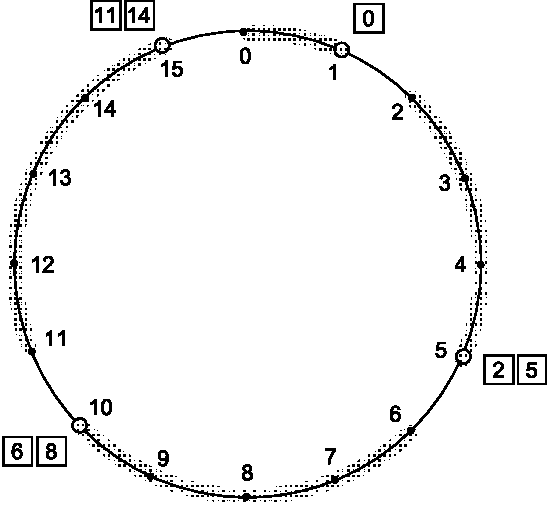
\includegraphics[width=0.4\textwidth]{pictures/pic0}\\
%  \caption[Example of a $4$-bit Chord identifier circle]{Example of a $4$-bit Chord identifier circle.
%  The responsibility ranges for each peer are accentuated in light gray}\label{fig:pic0}
%\end{figure}
%Es lassen sich auch mehrere Bilder nebeneinander platzieren wie z.B. in Abbildung
%\ref{fig:multipic} zu sehen ist.
%\begin{figure}[hpbt]
% \centering
%  %%----start of first subfigure----
%  \subfloat[FIFO size limited to 20 entries]{
%   \label{fig:multipic:a} %% label for first subfigure
%   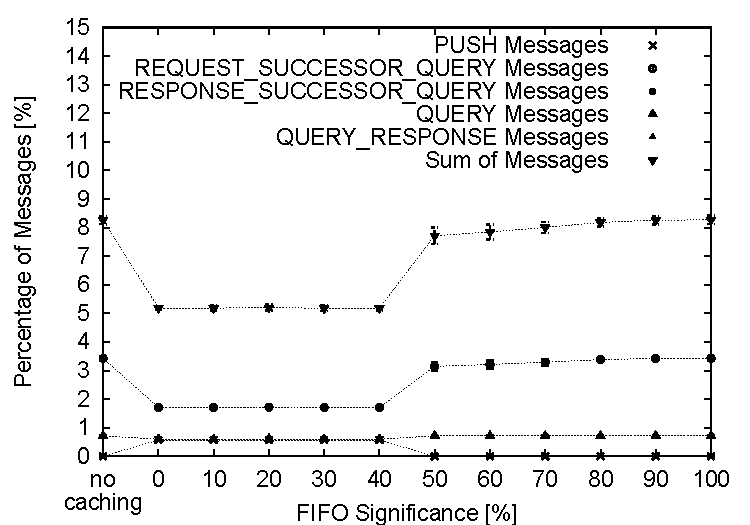
\includegraphics[width=0.48\linewidth]{pic1}}
%  \hspace{0.01\textwidth}
%  %%----start of second subfigure----
%  \subfloat[FIFO size limited to 30 entries]{
%   \label{fig:multipic:b} %% label for second subfigure
%   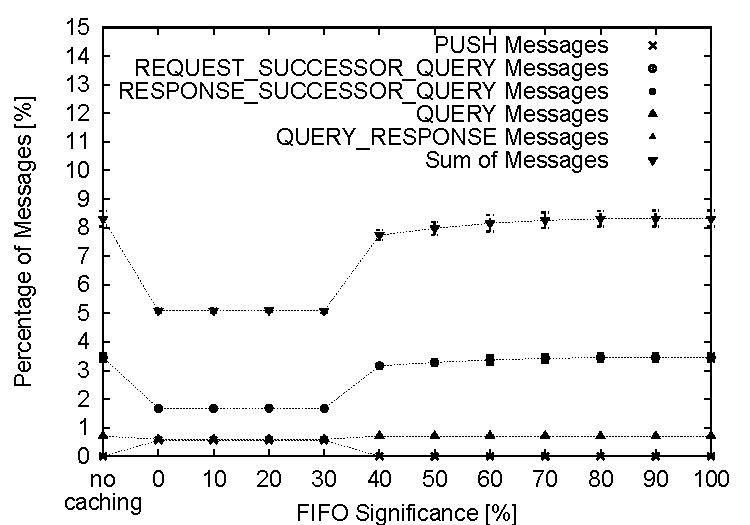
\includegraphics[width=0.48\linewidth]{pic2}}\\[0pt] % horizontal break
%  %%----start of third subfigure----
%  \subfloat[FIFO size limited to 40 entries]{
%   \label{fig:multipic:c} %% label for third subfigure
%   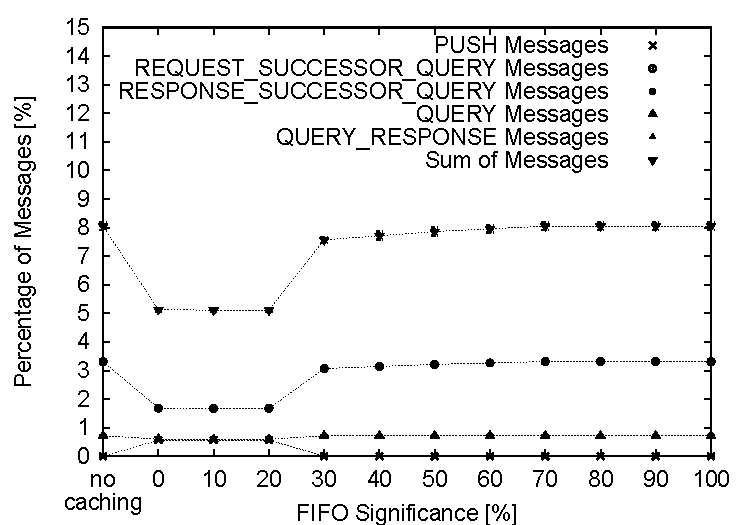
\includegraphics[width=0.48\linewidth]{pic3}}
%  \hspace{0.01\textwidth}
%  %%----start of fourth subfigure----
%  \subfloat[FIFO size limited to 50 entries]{
%   \label{fig:multipic:d} %% label for fourth subfigure
%   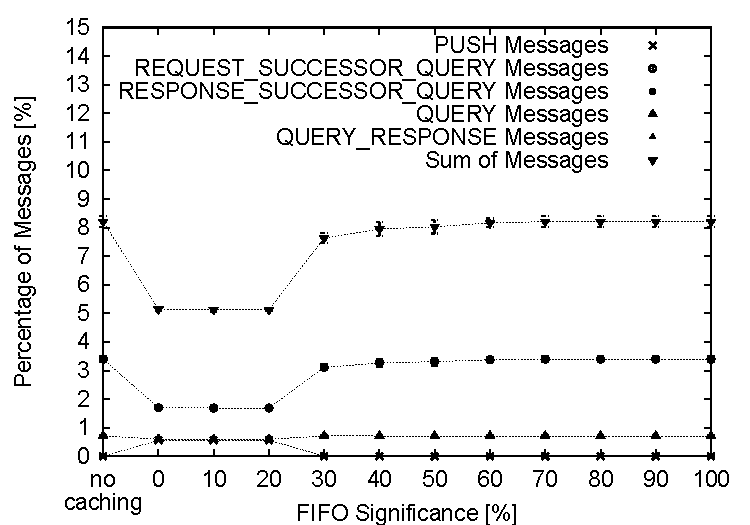
\includegraphics[width=0.48\linewidth]{pic4}}
% \caption[Observed message fractions and 95\% confidence intervals for Chord]{Observed message fractions and 95\% confidence intervals for Chord without the influence of churn. The FIFO capacity varies from 20 (\ref{fig:multipic:a}) -- 50 (\ref{fig:multipic:d}) entries (decadic steps).}
% \label{fig:multipic} %% label for entire figure
%\end{figure}
%
%\subsection{Programm Code}
%Eine elegante Möglichkeit, Programmtext einzubinden, lässt sich mit dem listings-Paket erreichen.
%Das \verb|HelloWorld| Programm aus Listing \ref{lst:hw} hat in Zeile \ref{line:hw3} übrigens einen Programmierfehler.
%\begin{lstlisting}[float=htp,caption=Hello World,label=lst:hw,language=Java, numbers=left, numberstyle=\tiny, stepnumber=2, numbersep=8pt, escapeinside={//@}{@//},backgroundcolor=\color{yellow},xleftmargin=3ex,xrightmargin=1ex]
%public class HelloWorld {
%    public static void main(String[] args) {
%        Syste.out.println("Hello, World"); //@\label{line:hw3}@//
%    }
%}
%\end{lstlisting}